\usetikzlibrary{arrows}
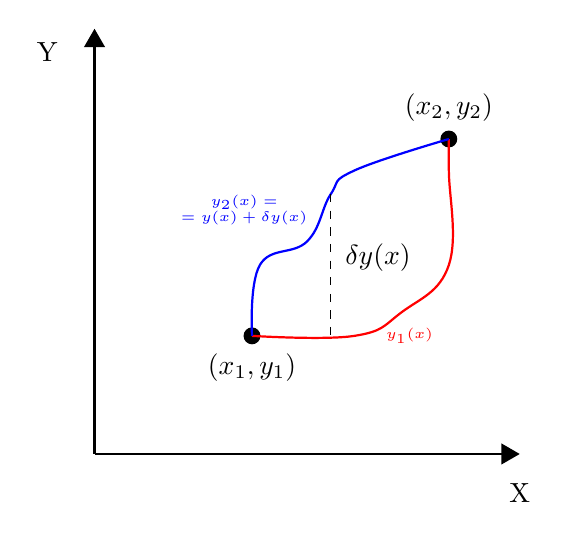
\begin{tikzpicture}



\draw [-triangle 60, thick](0,0) node (v1) {} -- (0,5.4);
\draw [-triangle 60, thick](0,0) node (v1) {} -- (5.4,0);
\node (p1) at (2,1.5) {};
\node at (p1) [below=3] {$(x_1,y_1)$};
\node (p2) at (4.5,4) {};
\node at (p2) [above=3] {$(x_2,y_2)$};
\draw [fill] (p1) circle [radius=0.1];;
\draw [fill] (p2) circle [radius=0.1];;



\draw [thick,red] plot[smooth, tension=.7] coordinates {(p1) (3.3,1.5) (3.9,1.8) (4.5,2.4) (4.5,3.6) (p2)};
\draw [thick,blue] plot[smooth, tension=.7] coordinates {(p1) (2.1,2.4) (2.7,2.7) (3,3.3) (3.3,3.6) (p2)};

\node at (5.4,-0.5) {X};
\node at (-0.6,5.1) {Y};
\draw [dashed](3,3.3) -- (3,1.5);
\node at (3.6,2.5) {$\delta y(x)$};

\node at (4,1.5) [red] {\tiny $y_1(x)$};

\node at (1.9,3.2) [blue] {\tiny $y_2(x)=$};

\node at (1.9,3) [blue] {\tiny $=y(x)+\delta y(x)$};
\end{tikzpicture}